\subsection{Cubrimientos pares}
\begin{definicion}
Sea \(p : \tilde{X} \to X\) una funcion continua sobreyectiva. El abierto \(U
\subseteq X\) se dice \textbf{parmente cubierto} por \(p\) si existe
\(\{V_\alpha\}_{\alpha \in \Lambda},\ \Lambda \subseteq \mathbb N\) tal que
\[ p^{-1} (U) = \bigcup_{\alpha \in \Lambda} V_\alpha \]
Donde \(\{V_\alpha\}\) es una familia disjunta de abiertos, tal que
\(\forall \alpha \in \Lambda, p \mid_{\alpha}\) es biyecctivo en \(U\).

Si para todo \(x \in X\) existe dicha vecindad \(U\) que cumpla lo
anterior, se dira que \(\tilde{X}\) es un \textbf{espacio cubrimiento} de \(X\)
y que \(p\) es un \textbf{cubrimiento par}.
\end{definicion}

Un ejemplo simple de espacio cubrimiento y cubrimiento par es \(p :
\mathbb R \to S^1,\ p(t) := e^{2 \pi \imath t}\). Este es claramente
sobreyectivo y continuo, escogiendo dos abiertos ejemplares como \(U =
S^1 - \{(1,0)\}\) y \(V = S^1 - \{(-1,0)\}\), es claro que
\[
    p^{-1} (U) = \bigcup_{n \in \mathbb Z} (n, n+1)
    \qquad p^{-1} (V) = \bigcup_{n \in \mathbb Z} (n - \frac 1 2, n + \frac 1
    2 )
\]
Donde estas familias de conjuntos son disjuntos y restringidos a cada
uno se tiene la inyectividad requerida.

A priori el cubrimientos par es irrespectivo de los caminos que tengamos
en \(X\), queremos ver si podemos reflejar la informacion importante de
estos en \(\tilde{X}\).
\begin{figure}[h]
  \centering
  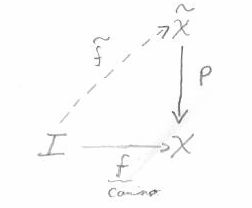
\includegraphics[scale=0.5]{./imagenes/lifting-path-diagrama.png}
\end{figure}
Para esto construiremos \(\tilde f : I \to \tilde X\) el cual cumpla \(p
\circ \tilde f = f \), veremos tambien que bajo hipotesis sensatas, este
\(\tilde f\) es unico y refleja informacion homotopica. Para esto
necesitamos desarrollar algunos teoremas previos.
\begin{lema}[Numero de Lebesgue] \label{thm:lebesgue-number-lema}
  Sea \(\mathcal A\) un cubrimiento del espacio metrico \((X,d)\). Si
  \(X\) es compacto, entonces existe \(\delta > 0\) tal que para todo
  subconjunto de \(X\) teniendo diametro menor que \(\delta\), existe un
  elemento de \(\mathcal A\) conteniendolo.
\end{lema}
\begin{proof}
  Supongamos que \(X \not \in \mathcal A\), pues si no trivialmente el
  teorema se cumple \(\forall \delta > 0\). Por compacidad de \(X\)
  existe una coleccion \(\{A_1,\dotsc,A_n\} \subset \mathcal A\) que
  cubre a \(X\), definamos a los conjuntos \(C_i = X - A_i,\ \forall i
  \in [1,n]\) y a la funcion \(f : X \to \mathbb R\) definida por
  \[ f(x) = \frac 1 n \sum_{i=1}^{n} d(x, C_i) \]
  ie la distancia promedio de \(x\) a \(C_i\). Notemos que \(\forall x,\
  f(x) > 0\), pues para \(x \in A_i \subseteq X\), por ser \(A_i\) un
  abierto, existe \(\epsilon > 0\) tal que \(B(x,\epsilon) \subset A_i\)
  y por tanto \(d(x, C_i) \geq \epsilon\) que implica  \( f(x) \geq \frac
  \epsilon n > 0\).

  Por otro lado \(f\) es una funcion continua sobre \(X\), un compacto,
  por lo tanto alcanza un minimo; a este le denotaremos como nuestro
  \(\delta\). Probaremos que este cumple el requerimiento, sea \(B
  \subset X\) subconjunto abierto de diametro menor que \(\delta\), sea
  \(x \in B\) arbitrario, el cual tiene tiene una vencindad contenida en
  \(B\) de diametro menor a \(\delta\). Dado que
  \[\delta \leq f(x) \leq d(x, C_m)
      \qquad d(x, C_m) = \max_{i \in [1,n]} d(x, C_i)\]
  Esto nos dice que dado \(\delta \leq d(x, C_m)\), existe una vecindad
  de al menos diametro \(\delta\) que contiene a \(x\) en \(X - C_m = A_m\).
\end{proof}
\begin{definicion}[Levantamiento de \(f\)]
  Sea \(p : \tilde X \to X\) un mapeo. Si \(f : W \to X\) es un mapeo
  continuo, un levantamiento de \(f\) es una funcion \(\tilde f : W \to
  \tilde X\) tal que \(p \circ \tilde f = f\).
\end{definicion}
Ver que la definicion es mucho mas general que lo que pediamos al
diagrama. Usualmente \(W = [0,1]\) pues estudiaremos los caminos sobre
\(X\). Veremos a continuacion teoremas de como se reflejan los caminos
y las homotopias en el espacio cubrimiento de \(X\).
\begin{teorema}
  Sea \(p : \tilde X \to X\) un cubrimiento par tal que \(p(\tilde x _0)
  = x_0 \), para algun \(\tilde x _0 \in \tilde X\). Para cualquier
  camino \(f : [0,1] \to X\) que comience en \(x_0\), tiene un
  unico camino levantamiento \(\tilde f\) en \(\tilde X\) que comienza
  en \(\tilde x _0\).
\end{teorema}
\begin{proof}
  Para todo punto de \(X\), existe una vecindad \(U_x\) que es
  cubierta parmente, por tanto \(\bigcup_{x \in X} U_x\) es cubrimiento
  de \(X\). Por otro lado, tenemos que \( [0,1] \subset p^{-1}
  (\bigcup_{x \in X} U_x)\). Por el Teorema
  \ref{thm:lebesgue-number-lema}, podemos elegir \(s_0,\dotsc,s_n\) tal
  que \(f([s_i, s_{i+1}])\) este contenido en algun \(U_x\). Definiremos
  \(\tilde f\) inductivamente.

  Primero declaremos \(\tilde f (0) = \tilde x _0\). Luego, suponiendo
  que \(\tilde f (s)\) esta definido para \(0 \leq s \leq s_i\), se
  define a \(\tilde f \) en \([s_i, s_{i+1}]\) de la siguiente forma.
  Dado que \(f ([s_i, s_{i+1}]) \subseteq U_x\) para algun \(x\) con
  \(U_x\) cubierto parmente por \(p\), denotemos a
  \(\{V_\alpha\}_{\alpha \in \Lambda} = p^{-1} (U_x)\). Debe de existir
  algun \(\alpha\) tal que \(\tilde f (s_i) \in V_\alpha\), a este le
  denotaremos \(V_0\). Dado que \(p \mid_{V_0}\) es un homeomorfismo,
  definimos a \(\tilde f (s)\) en \([s_i, s_{i+1}]\) por
  \begin{equation}
  \tilde f (s) = (p \mid _{V_0})^{-1} (f(s))\label{eq:tilde-f-inductiva}
  \end{equation}
  El cual es continuo en \([s_i, s_{i+1}]\) en virtud del lema del pegamiento.

  Para ver la unicidad, se probara inductivamente y por contradiccion.
  Supongamos que existe otro \(\tilde{\tilde f}\) levantamiento par de
  \(f\) que tambien comienza en \(x_0\), ie \(\tilde{\tilde f} (0) =
  \tilde x _0 = \tilde f (0)\). Supongamos que que \(\forall s \in [0,
  s_i],\ \tilde{\tilde f} (s) = \tilde f (s)\), dado que \(\tilde f\)
  esta definida por \eqref{eq:tilde-f-inductiva}
\end{proof}
